\chapter[综合案例二：识别并修正 AI 的系统性错误]{综合案例二：识别并修正 AI 在事故分析中的系统性错误}
\label{ch:case_two}

第 16 章展示了一个进展相对顺利的项目：错误被及时发现，返工被控制在可管理的范围内。本章选择一个方向相反的案例——一个 AI 特别容易出错、而且错误特别难以察觉的任务：利用道路交通事故数据分析严重事故的影响因素，并提出安全改善建议。

这类任务之所以“危险”，是因为它同时具备几个特点：数据字段多，其中混杂着事前信息、事后信息和由标签推导的字段；严重事故是少数类；标签的记录口径会随管理制度变化；而最终的问题——“怎么减少严重事故”——天然带有因果含义，很容易诱使 AI 把相关关系包装成政策建议。

本章沿用贯穿案例 B，使用英国交通部发布的 STATS19 道路交通伤亡事故数据（2021—2025 年，共 513,801 起事故）\cite{dft2026stats19}。与本书其他案例一样，本章报告的所有数字都由配套代码实际运行得到，主要脚本为 \texttt{code/case\_B\_crash/ch17\_error\_audit.py}。本章的组织方式是：先呈现 AI 的第一版分析，再按照第 12 章的错误分类逐项审查，每一项都说明错误的表现、发现方式、实测证据、修正方法，以及如何把这一教训写回下一版 Prompt。

学完本章后，读者应当能够：

\begin{itemize}
  \item 在一个真实数据集上识别数据性、统计性、技术性、领域性和幻觉性错误；
  \item 用可复现的对照实验量化每一类错误的影响，而不是凭印象判断；
  \item 区分“影响指标的错误”与“影响解释的错误”，理解后者往往更危险；
  \item 把错误检查的结果固化为 Prompt 约束和检查清单。
\end{itemize}

% ----------------------------------------------------------------
\section{任务与 AI 的第一版分析}
% ----------------------------------------------------------------

分析人员向 AI 提交了三张数据表（事故表、车辆表、伤亡人员表）和一句任务描述：

\begin{quote}
这是英国近五年的道路交通事故数据。请分析哪些因素导致了严重事故（死亡或重伤），建立一个预测模型，并据此提出减少严重事故的政策建议。
\end{quote}

为了便于讨论，本章把一个未经约束的 AI 分析流程——使用全部字段、随机划分、按常见默认做法建模和解读——可能给出的结论整理成一份“第一版报告”。报告中的每一个数字，都来自配套代码按这一流程在真实数据上的实际计算；报告的文字表述则代表了这类流程常见的解读方式。其要点可以概括为：

\begin{enumerate}
  \item 模型 Accuracy 和 ROC-AUC 均接近 1，“模型能够准确预测事故严重程度”；
  \item 最重要的因素包括调整后严重程度、事故伤亡人数和警员是否到场；
  \item 城市 30 mph 道路的严重事故数量最多，“是最危险的道路类型，应作为治理重点”；
  \item 限速每提高 10 mph，严重事故的优势比增加约 21\%，“建议普遍降低限速，预计可显著减少严重事故”；
  \item 近五年严重事故比例持续上升，“道路安全形势正在恶化”；
  \item 报告附有若干参考文献，以支持上述政策建议。
\end{enumerate}

这份报告中的每一个数字都来自真实计算，其表述方式也相当常见。但正如下文将要展示的，上述六条结论中没有一条可以原样采用。

% ----------------------------------------------------------------
\section{审查策略：从上游到下游}
% ----------------------------------------------------------------

第 12 章提出，检查应当先上游、后下游：先检查任务和数据，再检查实现和统计方法，最后检查结论与解释。原因很简单：上游的错误会让下游的一切检查失去意义——如果标签本身有问题，再精细的模型比较也只是在比较错误的东西。

分析人员据此把审查分为四层，并为每一层准备了一条 Prompt，要求 AI 先提供审查所需的事实，而不是评价自己的报告：

\begin{description}
  \item[数据层] 每个字段是在事故发生前可知、事故发生后产生、由标签推导，还是管理性字段？每行数据代表什么？
  \item[标签层] 标签如何产生？记录口径在时间和空间上是否一致？
  \item[方法层] 数据如何划分？类别变量如何编码？类别不平衡如何处理？
  \item[结论层] 每一条结论依赖什么证据？哪些是关联，哪些被表述成了因果？引用是否真实存在并支持相应论断？
\end{description}

% ----------------------------------------------------------------
\section{数据层的错误}
% ----------------------------------------------------------------

\subsection{错误一：由标签推导的字段进入了特征}

\paragraph{表现} 模型 Accuracy 与 ROC-AUC 均为 1.000，重要性排名第一的是 \texttt{collision\_adjusted\_severity\_slight}。

\paragraph{发现方式} “好得不可能”的结果本身就是最强的信号。第 12 章指出：越是高分和“符合预期”的结果，越值得检查。分析人员查阅 DfT 的数据说明后确认，\texttt{collision\_adjusted\_severity\_serious} 和 \texttt{collision\_adjusted\_severity\_slight} 是 DfT 为校正不同报告系统之间的差异、基于事故严重程度计算的调整概率\cite{dft2019severity}；\texttt{enhanced\_severity\_collision} 则是基于伤情系统给出的细分严重程度。

\paragraph{实测证据} 单独使用 \texttt{collision\_adjusted\_severity\_serious} 一个字段对 KSI 排序，ROC-AUC 即为 0.964；\texttt{enhanced\_severity\_collision} 单字段的 ROC-AUC 为 0.726。

\paragraph{修正与写回 Prompt} 删除全部标签派生字段。写回 Prompt 的约束是：“在建模前，逐一说明每个字段的产生方式；凡是由标签计算、或与标签同时由同一记录过程产生的字段，一律不得作为特征。”

\subsection{错误二：事故发生后才产生的信息进入了特征}

\paragraph{表现} 删除标签派生字段后，AI 保留了“警员是否到场”和“伤亡人数”，并把它们列为最重要的影响因素之一。

\paragraph{发现方式} 对照任务目的检查信息可得性。分析的目的是识别事故发生前可以干预的道路与环境条件；警员是否到场、伤亡人数都是事故发生后才确定的，而且在很大程度上是事故严重程度的结果而不是原因——严重事故更可能有警员到场处置。

\paragraph{实测证据} 在相同的时间划分（2021—2023 年训练，2025 年测试）和相同模型下，只用事前字段时 ROC-AUC 为 0.653、PR-AUC 为 0.412；加入这两个事后字段后，分别上升至 0.710 和 0.468。这部分“提升”完全来自不可能在事前获得的信息。

\paragraph{修正与写回 Prompt} 删除事后字段。约束写为：“特征只能是事故发生前可知的道路、环境、时间条件；若使用涉事方类型等条件变量，需在报告中说明其作用是分层解释，而不是事前预测。”

\subsection{错误三：多条记录对应同一起事故}

\paragraph{表现} 在一个补充分析中，AI 把车辆表与事故表合并，在“车辆”层面建模（加入驾驶人年龄、车辆类型、行驶动作等），并随机划分训练集与测试集。

\paragraph{发现方式} 检查“每行数据代表什么”。合并后，每起事故平均对应 1.50 条车辆记录，同一起事故的多条记录共享完全相同的事故级特征和标签。随机划分会使同一起事故的记录同时出现在训练集和测试集中。

\paragraph{实测证据} 在 2021—2023 年随机抽取的 40 万条车辆级记录上，随机划分的 ROC-AUC 为 0.686，按事故分组划分为 0.674。在本数据中虚高幅度不大，因为多数事故只涉及一两辆车。但幅度小不等于可以忽略：在每个分组包含大量重复记录的数据中（例如同一条道路、同一辆车的多次观测），这种泄露可以非常严重。正确的做法是始终按分析单元分组划分，而不是事后估计“泄露得多不多”。

\paragraph{修正与写回 Prompt} 约束写为：“请先说明每行数据的观测单位；若多行属于同一事故、同一路段或同一对象，划分数据时必须按该单位分组。”

% ----------------------------------------------------------------
\section{标签层的错误}
% ----------------------------------------------------------------

\subsection{错误四：把记录口径的变化当作安全形势的变化}

\paragraph{表现} AI 报告“近五年严重事故比例持续上升，道路安全形势正在恶化”。

\paragraph{发现方式} 追问标签是如何产生的。英国警方记录伤害严重程度有两类方式：一类由警员根据现场判断确定，另一类是基于伤情的报告系统（如 CRASH），由警员从规定清单中选择伤情，再由系统自动确定严重程度。DfT 指出，基于伤情的系统会影响重伤人数的水平和趋势，因此提供了调整后的严重程度，以便在不同地区和年份之间比较\cite{dft2019severity}。STATS19 中的 \texttt{collision\_injury\_based} 字段标记了每起事故所用的系统类型。

\paragraph{实测证据} 表~\ref{tab:ch17_reporting} 与图~\ref{fig:ch17_reporting} 显示，采用基于伤情系统记录的事故占比，从 2021 年的 49.6\% 上升到 2024 年的 58.8\%，并在 2025 年跃升至 86.5\%。在任一年份内，两类系统记录的 KSI 比例都相差约 7 至 9 个百分点。全体事故 KSI 比例的上升，有相当一部分来自报告系统构成的变化。

\begin{table}[H]
\centering
\caption{案例 B：不同报告系统下的 KSI 比例（STATS19，2021—2025 年）}
\label{tab:ch17_reporting}
\begin{tabular}{lcccc}
\toprule
年份 & 基于伤情系统的占比 & KSI 比例（警员判断） & KSI 比例（基于伤情） & 全体 KSI 比例 \\
\midrule
2021 & 49.6\% & 0.186 & 0.265 & 0.225 \\
2022 & 52.6\% & 0.192 & 0.274 & 0.235 \\
2023 & 53.7\% & 0.192 & 0.280 & 0.239 \\
2024 & 58.8\% & 0.197 & 0.285 & 0.248 \\
2025 & 86.5\% & 0.214 & 0.270 & 0.262 \\
\bottomrule
\end{tabular}
\end{table}

\begin{figure}[H]
  \centering
  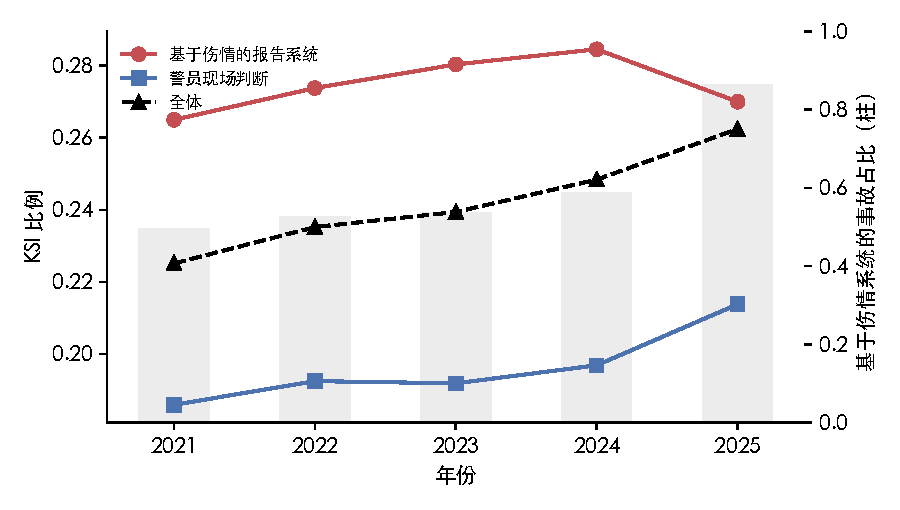
\includegraphics[width=0.72\textwidth]{figures/chapter17/reporting_system.pdf}
  \caption{案例 B：不同报告系统下的 KSI 比例（折线）与基于伤情系统记录的事故占比（柱），STATS19 2021—2025 年}
  \label{fig:ch17_reporting}
\end{figure}


这一变化对模型同样有直接影响。用 2021—2023 年数据训练的模型，对 2025 年事故的平均预测 KSI 概率为 0.214，而实际比例为 0.262。按报告系统拆开看：对基于伤情系统记录的事故，模型预测 0.209、实际 0.270，明显低估；对警员判断的事故，模型预测 0.252、实际 0.214，反而高估。模型学到的“风险水平”中，混入了训练期的报告系统构成。

\paragraph{修正与写回 Prompt} 趋势分析使用 DfT 的调整后严重程度，而不是原始 KSI 比例；建模时把报告系统类型作为分层变量，分别报告评价结果，并在部署前用最新年份数据重新校准概率。约束写为：“在解释任何时间趋势或地区差异之前，先检查标签的记录口径是否在时间和空间上一致。”

% ----------------------------------------------------------------
\section{方法层的错误}
% ----------------------------------------------------------------

\subsection{错误五：用 Accuracy 评价少数类问题}

第 8 章已经给出了这一错误的实测结果：在 2025 年测试集上，不加权逻辑回归的 Accuracy 为 0.738，与“把所有事故都判为非 KSI”的 Accuracy 完全相同，而 KSI 事故的 Recall 只有 3.3\%。修正方法是以 PR-AUC、分阈值的 Precision 与 Recall，以及“关注前 $k\%$ 能覆盖多少 KSI”这类决策指标为主，并把 Accuracy 仅作为参考。

\subsection{错误六：把类别编码当作连续数值}

\paragraph{表现} 在一版逻辑回归中，AI 把光照、天气、道路类型等整数编码直接作为数值特征输入，并报告“light\_conditions 的系数为 0.074，光照条件越差，严重事故风险越高”。

\paragraph{发现方式} 查阅编码表。光照条件的编码为 1（白天）、4（黑暗有路灯且亮）、5（黑暗有路灯未亮）、6（黑暗无照明）、7（光照未知），另有 $-1$ 表示缺失。“编码每增加 1”没有任何业务含义；编码 7（未知）甚至被模型当作比“黑暗无照明”更“黑暗”的状态。

\paragraph{实测证据} 这个错误对排序指标的影响很小：数值编码的 ROC-AUC 为 0.632，独热编码为 0.637。正因为如此，它很难从指标上被发现——模型“看起来差不多好”，但它给出的解释是错误的。本章开头 AI 报告中关于各因素影响方向的描述，有一部分就建立在这样的系数之上。

\paragraph{修正与写回 Prompt} 约束写为：“所有编码型字段按类别处理，并指定有业务含义的参照类别；‘未知’和缺失单独成类，不得与有效类别合并或按数值排序。”这一错误也提醒我们：检查 AI 的输出，不能只看指标有没有变差，还要看解释是否建立在正确的表示之上。

% ----------------------------------------------------------------
\section{结论层的错误}
% ----------------------------------------------------------------

\subsection{错误七：把数量当作风险}

\paragraph{表现} AI 报告“城市 30 mph 道路的严重事故数量最多，是最危险的道路类型”。

\paragraph{实测证据} 城市 30 mph 道路确实有最多的 KSI 事故（2021—2025 年共 50,947 起），但它同时有最多的事故（227,810 起），其 KSI 比例为 0.224，是各类道路中较低的；农村 60 mph 道路的 KSI 事故数为 21,125 起，KSI 比例却高达 0.348。更重要的是，无论数量还是比例，都没有考虑暴露量：城市 30 mph 道路承担了大量的交通量和出行，事故数量多，首先是因为在那里出行的人多。评价“哪类道路更危险”，需要的是单位交通量（例如每十亿车英里）的事故率，而这需要把 STATS19 与交通量统计数据结合起来——DfT 的年度道路安全统计报告正是这样计算伤亡率的。

\paragraph{修正与写回 Prompt} 约束写为：“比较不同道路、地区或时段的‘危险程度’时，必须说明使用的是数量、比例还是基于暴露量的比率；缺少暴露量数据时，不得使用‘最危险’一类表述。”

\subsection{错误八：把关联写成政策效果}

\paragraph{表现} AI 根据“限速每提高 10 mph，优势比为 1.21”，建议“普遍降低限速，预计可显著减少严重事故”。

\paragraph{发现方式} 追问这条结论的证据类型。优势比描述的是在其他纳入变量相同的条件下，不同限速道路上事故严重程度的关联，而不是“把同一条道路的限速降低”之后会发生什么。限速不是随机分配的：高限速道路往往是农村公路、快速路，道路几何、交通构成、行车速度分布和急救可达性都与低限速道路不同，这些因素并未全部进入模型。从关联到干预效果，需要的是因果推断的设计，例如带对照组的前后对比研究\cite{hernan2020causal}。

值得注意的是，“降低车速有助于减少严重伤亡”这一方向本身有大量交通安全研究支持。问题不在于结论的方向，而在于证据与表述不匹配：一个基于横截面关联的模型，被用来给出“预计可显著减少”这种带有干预效果含义的承诺。

\paragraph{修正与写回 Prompt} 结论被改写为：“在控制了道路类型、城乡、光照和涉事方类型后，较高的限速仍与较高的 KSI 比例相关；这一关联与交通安全文献中关于速度与伤害严重程度的结论方向一致，但本分析不能估计降低限速的效果，相关政策需以前后对比等评估设计为依据。”约束写为：“除非任务明确包含因果识别设计，否则结论只能描述关联，不得使用‘导致’‘预计减少’等因果或干预表述。”

\subsection{错误九：无法核实的参考文献}

\paragraph{表现} 报告为政策建议附上了若干参考文献。

\paragraph{发现方式与处理} 分析人员没有直接采用这些文献，而是逐条核对：通过 DOI 或出版社页面确认文献真实存在；确认作者、年份、期刊与 AI 给出的一致；阅读原文，确认它确实支持报告中的具体论断，而不是只在主题上相关。大语言模型可能生成格式完整、看起来可信但并不存在的引用，这一现象已在多个领域被反复记录\cite{ji2023survey}。2023 年，美国一起联邦诉讼中，律师提交的法律文书引用了由聊天机器人生成、实际并不存在的判例，法院随后对相关律师作出了制裁，这是这一风险在专业工作中造成实际后果的典型事例。

\paragraph{写回 Prompt} 约束写为：“不要生成参考文献列表；如需引用，只能引用我提供的文献或给出可检索的 DOI，并标注每条引用支持的具体论断。所有引用由人工核实后方可进入报告。”

\subsection{错误十：迎合使用者的预期}

在审查过程中，分析人员还做了一个小实验：用三种不同的措辞，请 AI 评价同一个结论“夜间无照明是最重要的风险因素”——第一种表达赞同，第二种表达怀疑，第三种保持中立。读者可以用配套数据自行重复这一实验。第 12 章讨论过的谄媚倾向\cite{sharma2023sycophancy}意味着，AI 的评价可能随着提问者表达的立场而改变。而在本案例的数据中，这一结论本身并不成立：随机森林的置换重要性和逻辑回归的优势比都显示，涉及摩托车或行人等涉事方因素的关联远强于光照条件（第 8 章）。防范这一风险的办法，是在请求审查时使用中立措辞，并要求 AI 先给出支持和反对某一结论的证据，再给出判断。

% ----------------------------------------------------------------
\section{修正后的分析}
% ----------------------------------------------------------------

经过上述修正，分析人员得到的是一份结论少得多、但每一条都有证据支持的报告。其核心内容如下：

\begin{enumerate}
  \item \textbf{预测能力有限但真实：}只使用事前可知的道路、环境与时间条件以及涉事方类型，模型在 2025 年测试集上的 ROC-AUC 为 0.653，PR-AUC 为 0.412（随机水平为 0.262）；按风险得分排名前 20\% 的事故覆盖了 32.6\% 的 KSI 事故。
  \item \textbf{主要关联因素：}涉及行人（优势比 2.86）、摩托车（2.69）、自行车（2.12）；农村道路（1.35）；夜间（1.36）；黑暗无照明（1.25）；限速每提高 10 mph（1.21）。环岛（0.59）和双幅路（0.73）与较低的 KSI 比例相关。
  \item \textbf{重要的限定：}KSI 比例的时间变化受报告系统构成变化的显著影响，趋势判断应使用调整后严重程度；上述关联不等于干预效果；“危险程度”的比较需要结合交通量等暴露数据。
  \item \textbf{建议的下一步：}将 STATS19 与道路交通量数据结合，计算基于暴露量的事故率；针对摩托车与弱势道路使用者相关的高风险条件，设计有对照组的改善措施评估方案。
\end{enumerate}

表~\ref{tab:ch17_summary} 汇总了本章讨论的全部错误。

\begin{table}[H]
\centering
\caption{案例 B：AI 分析中被发现的错误汇总}
\label{tab:ch17_summary}
\small
\begin{tabular}{p{3.4cm}p{1.5cm}p{3.6cm}p{4.4cm}}
\toprule
错误 & 类型 & 实测影响 & 发现方式 \\
\midrule
标签派生字段入模 & 数据性 & AUC 1.000（虚假） & 结果好得不可能；查阅数据说明 \\
事后字段入模 & 数据性 & AUC 0.653 $\rightarrow$ 0.710（虚高） & 对照任务目的检查可得性 \\
同一事故多行随机划分 & 数据性 & AUC 0.674 $\rightarrow$ 0.686（虚高） & 检查观测单位 \\
记录口径变化当作趋势 & 领域性 & 2025 年预测 0.214 vs 实际 0.262 & 追问标签如何产生 \\
用 Accuracy 评价少数类 & 统计性 & Acc 0.738，Recall 0.033 & 与“全判为负”比较 \\
编码当作连续数值 & 技术性 & AUC 几乎不变，解释错误 & 查阅编码表 \\
数量当作风险 & 领域性 & 数量第一的道路比例较低 & 区分数量、比例与暴露 \\
关联写成政策效果 & 领域性 & —— & 追问证据类型 \\
无法核实的引用 & 幻觉性 & —— & 逐条核对来源 \\
迎合使用者预期 & 幻觉性/谄媚 & —— & 改变措辞重复提问 \\
\bottomrule
\end{tabular}
\end{table}

这张表中有一个值得反复体会的规律：影响指标最大的错误（前两项）反而最容易被发现，因为它们产生了“好得不可能”的数字；而影响解释的错误（编码、口径、数量与风险、关联与因果）几乎不改变指标，却直接决定了报告会给出什么建议。一个只盯着模型分数的审查者，恰恰会漏掉后者。

% ----------------------------------------------------------------
\section{把教训写回 Prompt}
% ----------------------------------------------------------------

本章的每一个错误，最终都被转化为一条约束。把它们汇总在一起，就得到了一份可以在今后任何事故数据分析任务中复用的“公共约束”：

\begin{quote}
\textbf{【事故数据分析公共约束】}
\begin{enumerate}
  \item 建模前，逐一说明每个字段的产生方式，并分为：事前可知、事后产生、由标签推导、管理性字段。后三类不得作为特征。
  \item 说明每行数据的观测单位；若多行属于同一事故、路段或对象，按该单位分组划分数据。涉及时间的任务按时间划分。
  \item 说明标签的记录口径，检查其在时间和空间上是否一致；解释趋势或地区差异前，先排除记录口径变化的影响。
  \item 编码型字段按类别处理，“未知”和缺失单独成类，并指定有业务含义的参照类别。
  \item 少数类问题以 PR-AUC、分阈值 Precision 与 Recall 以及资源约束下的覆盖率为主要指标，并与“全部判为多数类”和简单规则比较。
  \item 比较危险程度时，说明使用的是数量、比例还是基于暴露量的比率。
  \item 除非任务包含因果识别设计，结论只描述关联，不使用因果或干预效果的表述。
  \item 不自行生成参考文献；引用须可检索并由人工核实。
  \item 对任何违反直觉的结果，先分组检查，再给出解释；给出解释时，同时列出支持和反对该解释的证据。
\end{enumerate}
\end{quote}

这份约束清单本身，就是本书书名“提示即代码”的一个具体体现：它像代码中的断言和测试一样，把过去的错误变成了未来的检查。

% ----------------------------------------------------------------
\section{本章小结}
% ----------------------------------------------------------------

\begin{itemize}
  \item 事故分析是 AI 特别容易出错的任务：字段混杂、少数类、标签口径变化，以及天然的因果诱惑。
  \item 影响指标最大的错误（标签派生字段、事后字段）最容易被发现；影响解释的错误（编码、口径、数量与风险、关联与因果）几乎不改变指标，却决定了报告的建议。
  \item 每一类错误都应通过可复现的对照实验量化其影响，而不是凭印象判断。
  \item 把全部教训写成可复用的“公共约束”，是“提示即代码”最直接的体现。
\end{itemize}

% ----------------------------------------------------------------
\section{实战练习}
% ----------------------------------------------------------------

\subsection*{练习一：复现与扩展}

运行 \texttt{code/case\_B\_crash/ch17\_error\_audit.py}，复现本章的全部数字。然后选择一个本章未讨论的字段（例如 \texttt{special\_conditions\_at\_site} 或 \texttt{carriageway\_hazards}），判断它属于哪一类字段，并说明理由。

\subsection*{练习二：设计暴露量分析}

查找 DfT 发布的道路交通量统计数据，设计一个把事故数据与交通量数据结合的分析方案，计算不同道路类型的单位交通量 KSI 事故率。说明两类数据在空间单位和时间单位上如何对齐，以及可能出现的对齐误差。

\subsection*{练习三：报告系统的敏感性分析}

分别只使用基于伤情系统记录的事故、只使用警员判断记录的事故，重新训练第 8 章的逻辑回归，比较两组优势比的差异。哪些因素的关联在两组中稳定，哪些不稳定？这对结论的可靠性意味着什么？

\subsection*{练习四：谄媚实验}

按照本章“错误十”描述的方式，设计三种措辞，请 AI 评价“夜间无照明是最重要的风险因素”这一结论，记录三次回答的差异，并用第 8 章的分析结果判断哪一次回答更接近证据。
